\chapter[eProbe: Sampling of Environmental DNA within Tree Canopies with Drones]{eProbe: Sampling of Environmental DNA within Tree Canopies with Drones}
\label{ch:EP}

\author{Steffen Kirchgeorg}
\affiliation[ERL]{Environmental Robotics Laboratory, ETH Zürich, Zürich, 8092, Switzerland}
\alsoaffiliation[WSL]{Swiss Federale Institute for Forest, Snow and Landscape Research WSL, Birmensdorf, 8903, Switzerland}
\email{skirchgeorg@ethz.ch}
%
\author{Jia Jin Marc Chang}
\affiliation[NUS]{Department of Biological Sciences, National University of Singapore, Singapore, 117558, Singapore}
\alsoaffiliation[LKC]{Lee Kong Chian Natural History Museum, National University of Singapore, Singapore, 117377, Singapore}
%
\author{Yin Cheong Aden Ip}
\affiliation[WA]{School of Marine and Environmental Affairs, University of Washington, Seattle, Washington, 98105, United States of America}
%
\author{Meret Jucker}
\affiliation[EDNA]{Environmental DNA, ETH Zürich, Zürich, 8092, Switzerland}
%
\author{Christian Geckeler}
\affiliation[ERL]{Environmental Robotics Laboratory, ETH Zürich, Zürich, 8092, Switzerland}
\alsoaffiliation[WSL]{Swiss Federale Institute for Forest, Snow and Landscape Research WSL, Birmensdorf, 8903, Switzerland}
%
\author{Martina Lüthi}
\affiliation[ELE]{Ecosystems and Landscape Evolution, ETH Zürch, Zürich, 8092, Switzerland}
%
\author{Enrico van der Loo}
\affiliation[EDNA]{Environmental DNA, ETH Zürich, Zürich, 8092, Switzerland}
%
\author{Elvira Mächler}
\affiliation[SimpleX]{SimplexDNA AG, Winterthur, 8404, Switzerland}
%
\author{Nicolás D. Franco-Sierra}
\affiliation[SYN]{Syndesis Health, Palm Beach Gardens, Florida, 33408, United States of America}
%
\author{Mailyn Adriana Gonzalez Herrera}
\affiliation[HUM]{Alexander von Humboldt Biological Resources Research Institute, Bogotá, 111311, Colombia}
%
\author{Lo\"{i}c Pellissier}
\affiliation[ELE]{Ecosystems and Landscape Evolution, ETH Zürch, Zürich, 8092, Switzerland}
\alsoaffiliation[WSL]{Swiss Federale Institute for Forest, Snow and Landscape Research WSL, Birmensdorf, 8903, Switzerland}
%
\author{Kristy Deiner}
\affiliation[EDNA]{Environmental DNA, ETH Zürich, Zürich, 8092, Switzerland}
\alsoaffiliation[SimpleX]{SimplexDNA AG, Winterthur, 8404, Switzerland}
%
\author{Andrea Desiderato}
\affiliation[PL]{Department of Invertebrate Zoology and Hydrobiology, Faculty of Biology and Environmental Protection, University of Lodz, Lodz, 90-136, Poland}
%
\author{Stefano Mintchev}
\affiliation[ERL]{Environmental Robotics Laboratory, ETH Zürich, Zürich, 8092, Switzerland}
\alsoaffiliation[WSL]{Swiss Federale Institute for Forest, Snow and Landscape Research WSL, Birmensdorf, 8903, Switzerland}
%

%%%%%%%%%%%%%%%%%%%%%%%%%%%%%%%%%%%%%%%%%%%%%%%%%%%%%%%%%%%%%%%%%%%%%
%% Some journals require a list of abbreviations or keywords to be
%% supplied. These should be set up here, and will be printed after
%% the title and author information, if needed.
%%%%%%%%%%%%%%%%%%%%%%%%%%%%%%%%%%%%%%%%%%%%%%%%%%%%%%%%%%%%%%%%%%%%%
\abbreviations{
eDNA, environmental DNA;
RC, remote controller;
BVLOS, beyond visual line of sight;
UAV, unmanned aerical vehicle;
COI, cytochrome c oxidase subunit I;
GLM, generalized linear model;
}
%
%\keywords{Biodiversity, eDNA, Surface Swabbing, Drone-Based Sampling}
%

%
%%%%%%%%%%%%%%%%%%%%%%%%%%%%%%%%%%%%%%%%%%%%%%%%%%%%%%%%%%%%%%%%%%%%%
%% The abstract environment will automatically gobble the contents
%% if an abstract is not used by the target journal.
%%%%%%%%%%%%%%%%%%%%%%%%%%%%%%%%%%%%%%%%%%%%%%%%%%%%%%%%%%%%%%%%%%%%%
%\newpage
\begin{abstract}
%
Environmental DNA (eDNA) analysis is a powerful tool for studying biodiversity in forests and tree canopies. However, collecting representative eDNA samples from these high and complex environments remains challenging. Traditional methods like surface swabbing or tree rolling are labor-intensive and require significant effort to achieve adequate coverage. This study proposes a novel approach for unmanned aerial vehicles (UAVs) to collect eDNA within tree canopies using a surface swabbing technique. The method involves lowering a probe from a hovering UAV into the canopy, collecting eDNA as it descends and ascends through branches and leaves. To achieve this, a custom-designed robotic system was developed, featuring a winch and a probe for eDNA collection. The design of the probe was optimized and a control logic for the winch developed to reduce the risk of entanglement while ensuring sufficient interaction force to facilitate transfer of eDNA onto the probe. The effectiveness of this method was demonstrated during the XPRIZE Rainforest Semi-Finals as ten eDNA samples were collected from the rainforest canopy and a total of 152 molecular operational taxonomic units (MOTUs) were identified using eDNA metabarcoding. We further investigate how the number of probe interactions with vegetation, the penetration depth, and the sampling duration influence the DNA concentration and community composition of the samples.%
\end{abstract}
%
%\vspace{-1cm}
\section*{Synopsis}
%\small
Environmental DNA collection in forests is labor-intensive and limited in reach. By collecting eDNA within tree canopies with drones, we detected 152 MOTUs and showed robotics’ potential to scale eDNA surveys.
%
%\newpage
%%%%%%%%%%%%%%%%%%%%%%%%%%%%%%%%%%%%%%%%%%%%%%%%%%%%%%%%%%%%%%%%%%%%%
%% Introduction
%%%%%%%%%%%%%%%%%%%%%%%%%%%%%%%%%%%%%%%%%%%%%%%%%%%%%%%%%%%%%%%%%%%%%
\section{Introduction}
\label{sec:intro}
%
\Gls{eDNA} analyses have emerged as a powerful tool in ecological research, revolutionizing our understanding of biodiversity and ecosystem dynamics \cite{deiner-2017, beng-2020}. Genetic material shed by organisms into their surrounding environment provides a non-invasive means of monitoring species presence and distribution. While traditionally studied in aquatic environments \cite{deiner-2017, lyet-2020, tsuji-2019}, many investigations have revealed the presence of \gls{eDNA} in terrestrial ecosystems, including the tree canopy \cite{valentin-2020, banerjee-2022, eDrone, macher-2023, allen-using-2023}. The ability to collect \gls{eDNA} from the surface of foliage and bark is particularly useful in ecosystems where water is not present or accessible, and it is expected to increase our ability to monitor and conserve biodiversity across landscapes.

Apart from direct release of genetic traces from plants and arboreal organisms, potential pathways for \gls{eDNA} to reach tree canopies may involve wind-mediated transport, deposition via precipitation, or animal-mediated transfer \cite{valentin-2021, lynggaard-2023}. Once deposited, \gls{eDNA} diffuses vertically into the understory and then into the soil through wind, rain or mist. Macher et al.\cite{macher-2023} exploited this natural diffusion process to collect \gls{eDNA} from rainwash and study invertebrate diversity in canopies. Alternatively, \gls{eDNA} must be actively collected from vegetation surfaces through swabbing \cite{lynggaard-2023}, touch \cite{eDrone}, surface-rolling \cite{valentin-2020, kyle-2022, peterson-2022, allen-sampling-2023} or spray aggregation \cite{valentin-2020, allen-2021}. Due to the few mechanisms facilitating \gls{eDNA} transport across terrestrial landscapes, \gls{eDNA} samples collected from vegetation are often localized and non-representative of larger areas \cite{valentin-2020, roger-2022}. Several sampling schemes use extrapolation to overcome these difficulties, but they still rely on a representative sample for a given area \cite{altermatt-2023}, which tends to be the logistically impractical aspect needing a resolution. This challenge is particularly pronounced in forest canopies, given the efforts and risks associated with operating above ground \cite{Nakamura2017, lowman-2012}. Therefore, applying these user-controlled sampling methods to tree canopies remains challenging. 

\begin{figure*}[tb]
% \begin{figure}[tb]
    \centering
    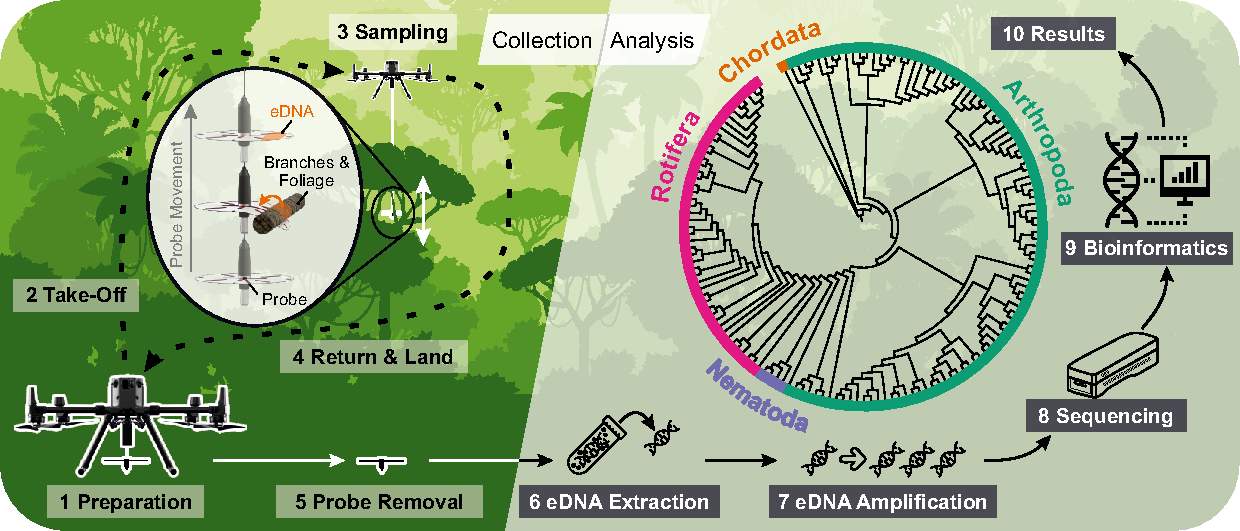
\includegraphics[width=\linewidth]{figures/01_overview.pdf}
    
    \caption{Overview of drone-based surface \gls{eDNA} sampling strategy and analysis in the lab. The drone is equipped with the probe (1) before take-off (2). The drone flies above the canopies to reach the sampling site (3), where the probe is lowered into the canopy and swabs against vegetation (inset) to collect \gls{eDNA}. The drone returns and lands (4). The probe is removed (5), and subsequently the DNA is extracted (6) and amplified (7) before sequencing (8). A bioinformatics pipeline (9) is employed to create the taxonomic assignments and results (10), here shown as a cladogram with the \glspl{MOTU} identified for all 10 collected samples during the XPRIZE Rainforest Semi-Finals.}
    \label{fig:1-intro}
% \end{figure}
\end{figure*}

Aerial robotics have significantly enhanced accessibility to tree canopies, facilitating remote data and sample collection with minimal effort and risk. Drones enable gathering physical samples of branches from tree canopies \cite{Charron2020}, retrieving endangered plant species from mountain cliff faces \cite{lavigne-2022}, and deploying sensors onto branches \cite{Geckeler2022, hamaza-2020}. Drone-based surface sampling of \gls{eDNA} has been proposed, involving landing on tree branches and collecting \gls{eDNA} through physical contact, i.e. “touch” \cite{eDrone}. This method relies on the availability of isolated and accessible tree branches, and it carries a high risk of collisions for the drone. To ensure greater safety and flexibility in collecting \gls{eDNA} across wide forested areas and inner canopy regions, alternative collection methods should be explored.

In this study, we propose a method for \glspl{UAV} to collect \gls{eDNA} within tree canopies based on surface swabbing (Fig.~\ref{fig:1-intro}), while keeping a safe operating distance from the vegetation. Our approach involves hovering above the canopy with a \gls{UAV}. Using a robotic winch, a specialized probe containing eDNA-retaining material, named the eProbe, is lowered into selected trees. As the eProbe descends and ascends, it collects environmental DNA by swabbing against branches and leaves (Fig.~\ref{fig:1-intro} inset). We optimized the design of the probe and developed a control logic for the winch to reduce the risk of entanglement while ensuring sufficient interaction force to facilitate transfer of \gls{eDNA} from the environment onto the collector material. We demonstrated the drone-based surface \gls{eDNA} collection from within rainforest canopies during the XPRIZE Rainforest Semi-Finals in Singapore in June 2023 by collecting 10 surface samples and extracting the DNA with battery-operated equipment, all within 24 hours. Then, \gls{eDNA} metabarcoding using the COI gene was performed. With the collected data, we examined the effect of the number of interactions between the probe and vegetation, the penetration depth of the probe in the canopy, as well as the sampling duration, on the DNA concentration and community composition of the collected samples.


%%%%%%%%%%%%%%%%%%%%%%%%%%%%%%%%%%%%%%%%%%%%%%%%%%%%%%%%%%%%%%%%%%%%%
%% Materials and Methods
%%%%%%%%%%%%%%%%%%%%%%%%%%%%%%%%%%%%%%%%%%%%%%%%%%%%%%%%%%%%%%%%%%%%%
\section{Materials and Methods}
\label{sec:methods}

\subsection{Sampling Methodology and System Design}
\label{sec:methods-probe}

Accessing terrestrial ecosystems, particularly forests, presents challenges due to the vegetation density, height, uneven terrain and remoteness \cite{Nakamura2017, lowman-2012}. Our sampling methodology therefore encompasses reaching and accessing these environments from above with the use of a UAV, and lowering a probe that penetrates the canopy to collect environmental samples. As the probe descends and ascends, it makes contact with vegetation, including branches and foliage. This movement and the physical contact with the vegetation generate a swabbing action that transfers genetic material from the environment to the probe (Fig.~\ref{fig:2-working-principle}). To retain \gls{eDNA} on the probe, a moisturized circular surface swab is used as the \gls{eDNA} collector material (Disko Lint-Free Fleece Cloths). The swab is reinforced radially with four interwoven fiberglass stiffeners to retain its shape and produce a swabbing action against the vegetation (Fig.~\ref{fig:2-working-principle}B). The probe is lowered using a tether (Spiderwire) from a robotic winch mounted on a DJI M300 drone (Fig.~\ref{fig:2-working-principle}C). The winch is driven by a Dynamixel XL330-M077T servomotor and controlled by an onboard computer. The pilot flies the drone over a tree of interest (Fig.~\ref{fig:2-working-principle}D) and activates the winch by sending commands through the \gls{RC}. The probe is automatically lowered into the canopy (Fig.~\ref{fig:2-working-principle}D) and swabs against vegetation on its descent and ascent (Fig.~\ref{fig:2-working-principle}E). A custom user interface is developed for the DJI RC to operate the winch, to select the length of the tether to be released from the winch to control the penetration depth in the canopy, and to provide feedback to the pilot on the winch status, tether length and force (see Supplementary Fig.~\ref{fig:s0-gui}). The flight time of the drone with the additional payload is 40 minutes.

\begin{figure*}[tb]
% \begin{figure}[tb]
    \centering
    \includegraphics[width=\linewidth]{figures/02_working_principle.pdf}
    \caption{Overview of eProbe surface sampling. (A) \gls{eDNA} collection schematic for descent and ascent of the probe with the transfer of \gls{eDNA}-particles from vegetation through touch, (B) Probe design with collector material, stiffeners and probe mount, (C) Complete drone sampling solution with winch, onboard computer and probe, (D) Image of the drone hovering and deploying the probe into the canopy, (E) Images showing the probe interacting with and swabbing the vegetation on the descent ($t=1s,3s$) and ascent ($t=14s,15s$).}
    \label{fig:2-working-principle}
\end{figure*}
% \end{figure}

During descent, the probe may encounter thick vegetation, causing it to rest on top of it and resulting in a slack tether. The ascent also presents challenges in thick vegetation, as the tension force on the tether increases, which can cause the winch to stall. A force sensor integrated in the winch monitors the tension force of the tether, and thus the control logic can automatically pull and release the probe to disentangle it from the vegetation. Details of the implementation of this control logic are provided in section \ref{sec:results-automation}. Furthermore, a safety release mechanism is incorporated to cut the tether in case the probe becomes irremovably entangled, ensuring the safety of the drone and surrounding environment.

The success of the collection process relies not only on the control strategy but also on the mechanical properties and geometry of the probe. Key factors in the efficacy of \gls{eDNA} collection include the probe's penetration capacity and swabbing force magnitude, both of which are influenced by its design. Deeper penetration, while maintaining retrievability, directly impacts coverage distance, thereby increasing the likelihood of encountering more surfaces for \gls{eDNA} collection. Furthermore, the interaction force between the probe and the environment generates the swabbing action necessary for transferring \gls{eDNA} onto the collector material. A softer-surfaced probe may penetrate vegetation more easily and be retrieved, but its swabbing action is reduced. Conversely, a stiffer probe can exert a higher interaction force, but its penetration capabilities are limited and it may become irretrievable. Therefore, we conducted a characterization of probe penetration, retrieval, and peak interaction forces across varying stiffness levels (refer to section \ref{sec:results-probe}). Additionally, we investigated the hypothesis that different locations of the collector material on the probe, relative to its center of mass, influence its penetration and retrieval. As the point of impact with the environment changes concerning the probe's center of mass and tether attachment point, we suspect a change in its behavior when traversing obstacles.


\subsection{Field Sampling at XPRIZE Rainforest Semi-Finals}
\label{sec:methods-sampling}

Field sampling was carried out as part of team ETH BiodivX’s participation in the XPRIZE Rainforest competition, a five-year-long competition aimed at developing technologies to rapidly assess biodiversity and enhance our understanding of rainforest ecosystems. The competition mandates that samples and data must be collected within 24 hours, without any human access to the survey site. The survey site was situated within the Singaporean Central Catchment Nature Reserve (Supplementary Fig.~\ref{fig:s1-sample-location}). Surface \gls{eDNA} samples were collected during the semi-finals testing window from June 5\textsuperscript{th} – 6\textsuperscript{th} 2023. In total, 10 samples were collected during 10 flights between June 5\textsuperscript{th} 1.18 pm and June 6\textsuperscript{th} 6.00 am, with five samples collected during the day and five during the night. Total sampling duration was 112 minutes. All flights were teleoperated and mostly \gls{BVLOS}.

The surface swabs were decontaminated through UVC exposure for 30 minutes and packaged and sealed individually in a dedicated clean lab prior to fieldwork. The swabs were attached to the probe and moisturized with molecular biology-grade water immediately before the drone sampling flight. A sample blank (ES000b) was taken by flying into the competition area and returning without lowering the probe. The sample blank underwent normal analysis like any other surface swab.

The extraction of the samples was done using portable laboratory equipment. The swabs were manually removed from the drone, and the fiberglass stiffeners were detached. Using sterilized tweezers, the swab was placed in a 50 mL forensic grade and certified DNA-free Eppendorf Conical Tube containing 7 mL of buffer (molecular biology grade water). To ensure the swab was fully submerged in the buffer, the conical tube was shaken by hand for several seconds. Subsequently, using the same tweezers, the swab was transferred to a 60 mL syringe, and any excess liquid was squeezed back into the original sample tube. DNA from the samples was extracted using a rapid extraction protocol. 1 mL aliquots were created and then stored in a fridge at 4°C in a designated ranger station in the Central Catchment Nature Reserve and two days later transported in a cool box to the National University of Singapore for preservation at -80 °C and subsequent analysis.

\subsection{eDNA Sample Analysis}
\label{sec:methods-edna}

For the metabarcoding assay, two length fragments of the cytochrome c oxidase subunit I (COI) gene were amplified. The first was the 658 bp Folmer region of COI, which was amplified using the primer pair LCO1490: 5'-GGT CAA CAA ATC ATA AAG ATA TTG G-3' and HCO2198: 5'-TAA ACT TCA GGG TGA CCA AAA AAT CA-3'\cite{folmer-1994}. The PCR primers had an additional 13 bp custom tag sequence on their 5’-end to allow for downstream demultiplexing \cite{meier-2016, srivathsan-2019} (see Supplementary File S1 for demultiplexing information). Three PCR replicates were performed for each surface sample, and each replicate had unique forward and reverse tag combinations (Supplementary File S1). Each PCR mix consisted of 5 µL of template DNA, 2 µL each of 10 µM tagged primers, 1 µL of bovine serum albumin (1 mg/mL), 1 µL of magnesium chloride (25 mM), 12.5 µL of GoTaq Green Master Mix (Promega), and was topped up to 25 µL with nuclease-free water. The thermocycling conditions were as follows: 94°C for 5 min, followed by 35 cycles of 94°C for 30 s, 42°C for 60 s, 72°C for 60 s, and a final extension for 5 min at 72°C. Additionally, we utilized the mlCOIintF: 5'-GGW ACW GGW TGA ACW GTW TAY CCY CC-3' \cite{leray-2013} and LoboR1: 5'- TAA ACY TCW GGR TGW CCR AAR AAY CA-3' \cite{lobo-2013} primer combination to amplify the 313 bp region of COI. No changes were made to the reaction mix and thermocycling conditions, but the mlCOIintF and LoboR1 primers were tagged with 8 bp tags instead. To maintain strict contamination control measures, all PCRs were prepared in a dedicated biosafety cabinet, and all working surfaces and laboratory equipment were sterilized with 20\% household bleach in ultrapure water, followed by UVC irradiation for at least 30 min before use. Amplification success was verified on 2\% agarose gels stained with GelRed (Biotium Inc.).

The amplicons were then pooled into two pools (658 and 313 bp), and cleaned using a 0.9 × ratio of AMPure XP beads (Beckman Coulter). Two libraries were prepared using the Ligation Sequencing Kit (SQK-LSK114) following the manufacturer’s protocols. Sequencing was performed on two R10.4.1 MinION flow cells; a fresh flow cell was used for sequencing both the 658 and 313 bp amplicon libraries, pooled in equimolar ratios; while the second was a previously washed flow cell ($\sim$ 500 available pores) and contained only the 658 bp library. Sequencing was performed on MinKNOW v23.07.12, for approximately 51 h per flow cell. The output pod5 files were subsequently basecalled on computer servers with Dorado v0.5.1 \cite{dorado}, using the dna\_r10.4.1\_e8.2\_400bps\_sup@v4.3.0 model.

Our bioinformatics pipeline was modeled after Chang et al.\cite{chang-2023}. Briefly, the basecalled-fastq files were first filtered using chopper v0.7.0 \cite{coster-2023} to retain only reads with $\geq 12$ Phred quality score (Q). Sequence reads were then demultiplexed to replicates with ONTbarcoder v2.1.3 \cite{srivathsan-2024} at default settings, and triplicates were concatenated to samples with custom bash scripts. Initial tests included additional gDNA treatments such as inhibitor removal (Zymo) on selected samples before PCR; these PCRs would have their own unique tag combinations, but were ultimately combined by sample for analysis (Supplementary File S1). Metabarcode consensus sequences were generated for each sample with amplicon\_sorter v2023-06-19 \cite{vierstraete-2022}, where demultiplexed reads were collapsed into a consensus sequence if they were $\geq 97 \%$ similar (--similar\_species), and consensus sequences were further combined if they were $\geq 98 \%$  similar (--similar\_consensus). The minimum and maximum lengths were set to $\pm 20$ bp of each expected amplicon length, and a 10× random sampling (--maxreads) was performed to increase the likelihood of sampling rare reads. Subsequently, all consensus sequences from both datasets were aligned with MAFFT v7.520 \cite{katoh-2013} with default settings, and further collapsed into \glspl{MOTU} with the objective clustering algorithm \cite{obj-cluster}. The program groups sequences based on a priori p-distance thresholds, where cluster members are separated from members of other clusters by tested p-distance thresholds \cite{meier-2006}. The commonly-used 3\% threshold was used to delimit species. \glspl{MOTU} were subjected to command line blastn (in NCBI BLAST+ v2.13.0 \cite{camacho-2009}, e-value: 1e-10) against an \textit{nt} database (last updated 21 JAN 2024). Blast hits were parsed through readsidentifier v1.1.2 \cite{srivathsan-2015} in order to obtain taxonomic classifications for the best blast hit for each \gls{MOTU}; we set the minimum identity threshold at 85\% and the minimum overlap to be 90\% of the amplicon length (i.e., 281 bp and 592 bp for short and long COI amplicons, respectively). Only \glspl{MOTU} classified as ‘Metazoa’ were retained. Additionally, all Metazoa \glspl{MOTU} found in the field blank (see Supplementary\_File\_S2, sheet "MOTUs\_omitted") and PCR negatives were removed from the corresponding surface samples prior to any statistical analyses. Due to the small sample size, the short and long COI datasets were combined by probe sample for further community analysis.

Community \gls{eDNA} analyses were performed in R4.3.3. The relationship between number of eProbe samples and \gls{MOTU} richness was examined with iNEXT v3.0.0 \cite{hsieh-2016}. The multicollinearity between the metadata variables relative to the sampling (i.e., sampling duration, number of touches with vegetation, maximum depth and mean maximum sampling depth; see Table 1) was checked using ggpairs in GGally v2.2.1 \cite{ggally}. The analysis also included the DNA concentration. To test the effect of the sampling on DNA concentration and \gls{MOTU} richness (i.e., our main response variables to assess the effectiveness of sampling), these were modeled with a generalized linear model using glmmTMB of glmmTMB v1.1.8 \cite{brooks-2017} with Gaussian and Gamma distributions respectively using one variable per time. Final models (Supplementary Table~\ref{tab:s1-permancova}) were validated by simulating their residuals using the package DHARMa \cite{hartig-2022}. We also assessed community differences between probe samples via permutational multivariate analysis of covariance (PERMANCOVA), using the adonis2 function in vegan v2.6.4 \cite{oksanen-2022}. Samples were grouped by sampling time including the DNA concentration as covariable for PERMANCOVA. Community differences were finally analyzed and visualized with a distance-based redundancy analysis (dbRDA) using the CAPSCALE function in vegan; the duration of the sampling, the number of touches between the probe and the vegetation, mean maximum depth reached by the probe during the descent, and DNA concentration were included as predictors. For both analyses, the Jaccard similarity coefficient \cite{jaccard-1901} was used.


%%%%%%%%%%%%%%%%%%%%%%%%%%%%%%%%%%%%%%%%%%%%%%%%%%%%%%%%%%%%%%%%%%%%%
%% Results
%%%%%%%%%%%%%%%%%%%%%%%%%%%%%%%%%%%%%%%%%%%%%%%%%%%%%%%%%%%%%%%%%%%%%
\section{Results and Discussion}
\label{sec:results}

\subsection{Probe Design Characterization}
\label{sec:results-probe}

We studied the effect of the probe stiffness and geometry on the penetration capacity and peak interaction force between the probe and the vegetation in a controlled laboratory setup by varying the thickness of the fiberglass stiffeners (low - $t_1 = 0.2mm$; medium - $t_2=0.3mm$; high - $t_3=0.5mm$), as well as the location of the collector material on the probe mount (top, middle, bottom). The experimental setup in Fig.~\ref{fig:3-probe-results}A was used with two beams ($d_{beam}=4mm$) spaced $1/3$ and $2/3$ of the probe diameter apart, i.e. $w=5cm$ and $w=10cm$. The winch with the probe was mounted aligned with the center of the beams. The probe ($m = 60g$) was accelerated to maximum velocity downwards ($v_{down,max} = 100 cm/s$) as well as upwards ($v_{up,max} = 68 cm/s$). The success rates for overcoming the obstacles are shown in Fig.~\ref{fig:3-probe-results}B.

\begin{figure*}[tb]
% \begin{figure}
    \centering
    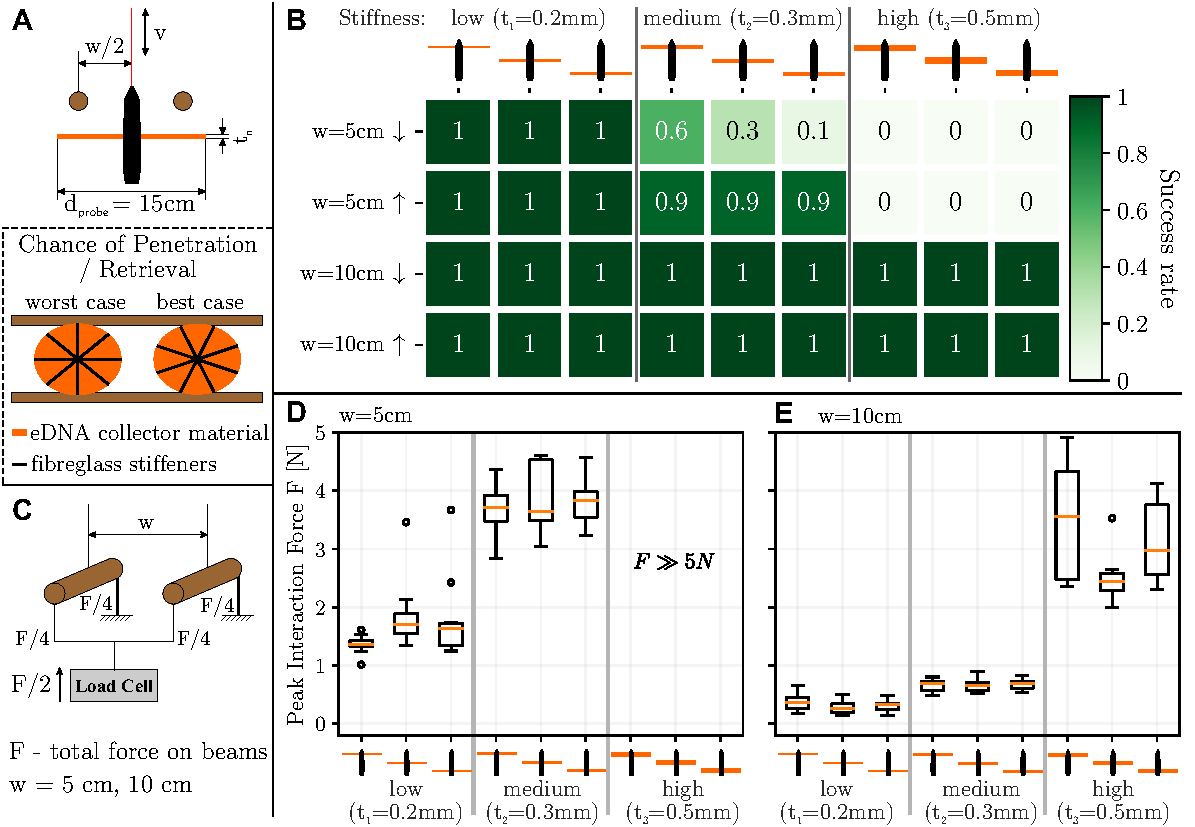
\includegraphics[width=\linewidth]{figures/03_eprobe_results_combined.pdf}
    \caption{Probe characterization. (A) Experimental setup for penetration and retrieval tests with inset showing worst and best case probe orientation, (B) Success rate (n=10) for the probe passing an obstacle for different probe stiffnesses (low $t_1$, medium $t_2$, high $t_3$), material locations (top, middle, bottom) and obstacles spaced $w=5cm, 10cm$ apart, for ascent and descent (C) Experimental setup with a load cell to measure the peak interaction force of the probe with the beams during the ascent and (D) Peak interaction force of the probe with the obstacles spaced $w=5cm$ and $w=10cm$ apart for different probe stiffness (low $t_1$, medium $t_2$, high $t_3$) and collector material location (top, middle, bottom) for upward motion.}
    \label{fig:3-probe-results}
% \end{figure}
\end{figure*}

Only the low stiffness probe ($t_1=0.2mm$) was able to overcome the closely spaced obstacles on descent and ascent, while the medium stiffness probe ($t_2=0.3mm$) struggled with descent as the probe would get stuck between the beams. The high stiffness probe could not overcome the obstacle at all. It was observed that due to the $\ang{45}$ arrangement of the fiberglass stiffeners, the probe would pass the obstacles more easily when the stiffeners were not perpendicular to the beams  (Fig.~\ref{fig:3-probe-results}A inset). During the experiment and sampling, the probe orientation cannot be controlled as the tether twist allows a rotation of the probe around its central axis. Therefore, multiple subsequent attempts can enable the probe to acquire an orientation that facilitates overcoming the obstacle  (Fig.~\ref{fig:3-probe-results}A inset, best case). Moreover, the data suggests that during ascent the probe gets stuck less than during descent, which would ensure that the probe only penetrates vegetation that it can also be retrieved from.
%
This is plausible as the winch can actively pull the probe upwards and exert a force, whereas downward motion and penetration rely on the probe's weight.
%
%
Despite some differences in success rate for different locations of collector material for probe $t_2=0.3mm$, no clear conclusion can be drawn between collector material placement and the probe passing success rate. For obstacles spaced wider apart ($w=10cm$), all probes passed the obstacles with ease. The motor and thus the maximum upward and downward velocities as well as the size of the surface swab were fixed. Nevertheless, the effectiveness of penetration and retrieval also depends on these system parameters. Therefore, conducting a more comprehensive analysis of motor speed, acceleration, torque as well as surface swab size would enable further optimization of the system.

\subsection{Winch Automation}
\label{sec:results-automation}

The control logic developed to automate the winch and to maximize vegetation penetration and retrieval is illustrated in Fig.~\ref{fig:4-control}A. During the experiments, it was observed that even slight changes in position may result in overcoming obstacles, both during descent and ascent. By detecting these impacts on the way down as well as the entanglements on the way up, we can initiate actions to overcome obstacles. By taring the force sensor to the weight of the probe ($m = 60g$) and introducing an impact threshold $F_i < -0.55N$ and an entanglement threshold $F_e > 1.5N$, it is possible to detect either downward impacts or upward entanglements (Fig.~\ref{fig:4-control}C). When a downward impact is detected, the probe is raised slightly, causing a small shift in its position, before trying to penetrate the vegetation again. A sequence of images illustrating this behavior is shown in Fig.~\ref{fig:4-control}B. If the obstacle can not be overcome on the way down after five attempts, the probe is retracted back to the drone (“Handle Impact” in Fig.~\ref{fig:4-control}A). Similarly, when an upward entanglement is detected, the probe is lowered slightly before accelerating the probe upward again (“Handle Entanglement” in Fig.~\ref{fig:4-control}A). If the probe cannot penetrate the vegetation upward and thus disentangle itself, additional operator intervention is required. %
%
The operator can retry to overcome the vegetation with the previously mentioned approach, but the force the motor can actively continuously pull saturates around \SI{2.5}{\newton}. However, the static force at which the motor overloads is almost three times higher (\SI{6.9}{\newton} with 40m spooled-up wire and $d_{spool+wire} = \SI{74}{\milli\metre}$). Therefore, this force can be applied by the drone as it is together with the weight of the system (\SI{6.9}{\newton}) well below the drone's payload limit (\SI{2.7}{\kilo\gram}, ~\SI{26.5}{\newton}). By raising the altitude of the drone, the operator can therefore exert additional force to overcome and free the probe from the vegetation. If neither of these solutions renders the probe free and thus safe to be retracted, a safety release mechanism can be activated, which cuts the tether and results in loss of the probe. While this leads to an unsuccessful sampling, it ensures the safety of the drone.

%If the probe cannot penetrate the vegetation upward and thus disentangle itself, additional operator intervention is required. The operator can retry to overcome the vegetation with the previously mentioned approach, but the static force the motor can apply saturates at \SI{2.5}{\newton}. Instead, the drone can exert a 10-times higher force as its payload limit is \SI{2.7}{\kilo\gram} (~\SI{26.5}{\newton}). By raising the altitude of the drone, the operator can exert additional force to overcome and free the probe from the vegetation. %
%With the motor under torque, a slightly larger force can be applied, but the motor gearing may break if the applied torque greatly exceeds the stall torque. Therefore, it is possible to deactivate the torque of the motor (i.e. a free-spinning mode) and let the spool unwind until the end of the wire, where it is fixed with a rubber band to the spool. As the rubber band breaks at \SIrange{24}{26}{\newton}, this is the maximum force exertable to free the probe, while keeping the drone safe. %
%However, it may not be desirable to unspool all the wire. Therefore, an active safety release mechanism is implemented, which cuts the tether and results in the loss of the probe. While this leads to an unsuccessful sampling, it ensures the safety of the drone.

\begin{figure*}[tbh]
% \begin{figure}[tb]
    \centering
    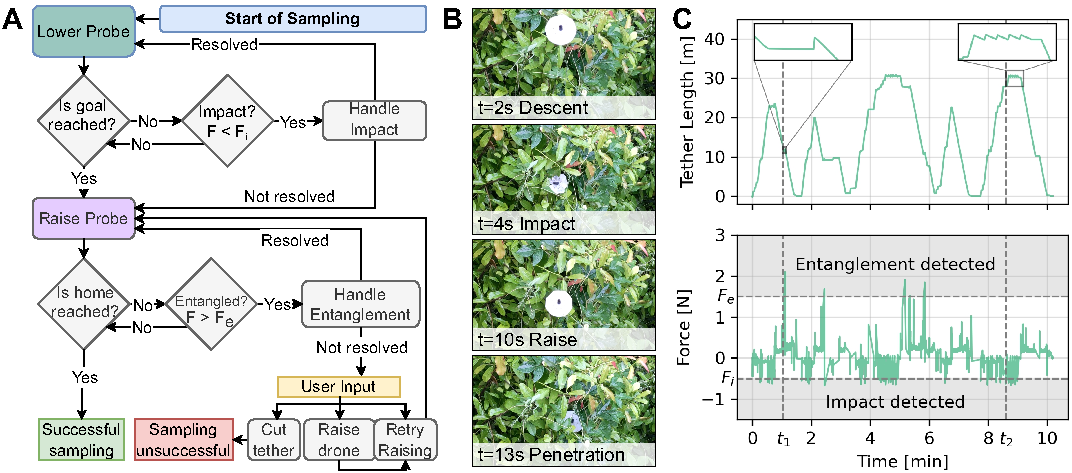
\includegraphics[width=\linewidth]{figures/04_control.pdf}
    \caption{(A) Control logic to detect and handle impacts and entanglements, (B) Sequence showing the probe impact dense vegetation, being raised and eventually penetrate through the vegetation, (C) Tether length and interaction force for surface probe ES006e with impact and entanglement thresholds, $F_i$ and $F_e$ respectively.}
    \label{fig:4-control}
% \end{figure}
\end{figure*}

\subsection{In-Field Data for eProbe}
\label{sec:results-field-data}

\begin{table*}[tb]
  \footnotesize
  \centering
  \caption{Summary of eProbe sample metadata and \gls{eDNA} results. Probes ES007e and ES0010e were not deployed, while data logging issues occurred during deployment of ES003e. The total \gls{MOTU} richness accounts for unique \glspl{MOTU} only (multiple detections across samples are ignored). Concentrations below 0.005 ng/µl are marked as “too low”.}
    \begin{tabular}{llcccccccc}
    \toprule
    \thead{Probe \\ Name} 
    & \thead{Start \\ Time}
    & \thead{Sampling \\ Duration \\$[min]$}
    & \thead{Down-\\Up\\Cycles\\$[\#]$}
    & \thead{Max.\\Sampling\\Depth\\$[m]$}
    & \thead{Mean\\Max.\\Sampling\\Depth $[m]$}
    & \thead{Touches\\$\vert F \vert$ \\$>0.5N$\\$[\#]$}
    & \thead{Dis-\\entangle-\\ments\\$[\#]$}
    & \thead{DNA\\conc.\\$[ng/\mu L]$}
    & \thead{Metazoan\\MOTU\\richness} \\
    \midrule
    ES001e & 1.18 pm & 10.10 & 9 & 20.7 & 13.58 & 95 & 5 & 0.0142 & 13 \\
    ES002e & 2.19 pm & 18.04 & 8 & 31.3 & 20.85 & 183 & 10 & 0.0180 & 15 \\
    ES003e & 4.06 pm & \multicolumn{6}{c}{Data logging malfunction} & Too low & 10 \\
    ES004e & 5.26 pm & 10.93 & 10 & 35 & 18.75 & 60 & 6 & 0.0148 & 14 \\
    ES005e & 7.00 pm & 9.44 & 5 & 25.4 & 19.30 & 50 & 3 & Too low & 4 \\
    ES006e & 1.37 am & 9.59 & 5 & 30.9 & 25.52 & 70 & 5 & 0.0764 & 35 \\
    ES008e & 3.28 am & 21 & 3 & 39.3 & 39.33 & 228 & 7 & 0.1680 & 55 \\
    ES009e & 4.25 am & 6.18 & 2 & 35.2 & 29.75 & 71 & 0 & 0.0820 & 38 \\
    ES011e & 5.00 am & 13.83 & 3 & 40.1 & 39.80 & 158 & 11 & 0.1230 & 32 \\
    ES012e & 5.43 am & 12.97 & 4 & 34.2 & 32.13 & 69 & 3 & 0.1240 & 22 \\
    \midrule
    \multicolumn{2}{r}{Total} & 112.09 & 49 & - & - & 984 & 50 & - & 152 \\
    \multicolumn{2}{r}{Average} & 12.45 & 5.90 & 31.60 & 26.56 & 103.33 & 5.56 & - & -\\
    \bottomrule
    \end{tabular}%
  \label{tab:1-metadata}%
\end{table*}%

Sample metadata is summarized in Table~\ref{tab:1-metadata} together with DNA concentration and \gls{MOTU} richness. The sampling duration describes the duration the probe was released into the canopy, while the down-up cycles show how often the probe was lowered during the sampling duration. Alongside this, the maximum sampling depth (from UAV altitude) is shown and mean maximum sampling depth across down-up cycles is computed. The amount of touches with surrounding surfaces is counted through a force threshold ($\vert F \vert > \SI{0.5}{\newton}$) and the number of disentanglements is noted. No unsolvable entanglement occurred during which the tether had to be cut, but the drone had to be raised 2-3 times to free probes.
In Figure~\ref{fig:4-control}C, we present a sample dataset detailing tether length and force values over time for sample ES006e (see Supplementary Figure~\ref{fig:s2-metadata} for other samples). The probe was lowered a total of 5 times at a single location (Supplementary Fig.~\ref{fig:s1-sample-location}). Analysis of the tether length suggests that during the 3\textsuperscript{rd} and 5\textsuperscript{th} cycle the ground was reached at around 30.9 meters from UAV altitude. At this tether length, subsequent impacts were observed that could not be resolved (Fig.~\ref{fig:4-control}C zoom-in top right), suggesting that either very dense vegetation or the forest floor was reached. Over the course of the sampling, several other impacts were observed as the force falls below \SI{-0.55}{\newton}. In addition, during upward motion, a total of 5 tether entanglements have been recorded with the tether force exceeding \SI{1.5}{\newton} A short stop and increase in tether length (Fig.~\ref{fig:4-control}C zoom-in top left) can be seen as the control logic (Fig.~\ref{fig:4-control}A) tries to disentangle the probe. For this probe, a total of 70 touches resulted in a DNA concentration of 0.0764 ng/uL, from which 35 metazoan \glspl{MOTU} were identified.
The system was able to successfully sample down to 40.1 meters (ES011e) from drone altitude and the data (Supplementary Figure~\ref{fig:s2-metadata}) further suggests that the probe impacted the forest floor for samples ES006e, ES008e and ES009e, thus penetrating through all forest strata.

\subsection{eDNA Community Results}
\label{sec:field-edna}

% \begin{figure}[tb]
\begin{figure*}[tb]
    \centering
    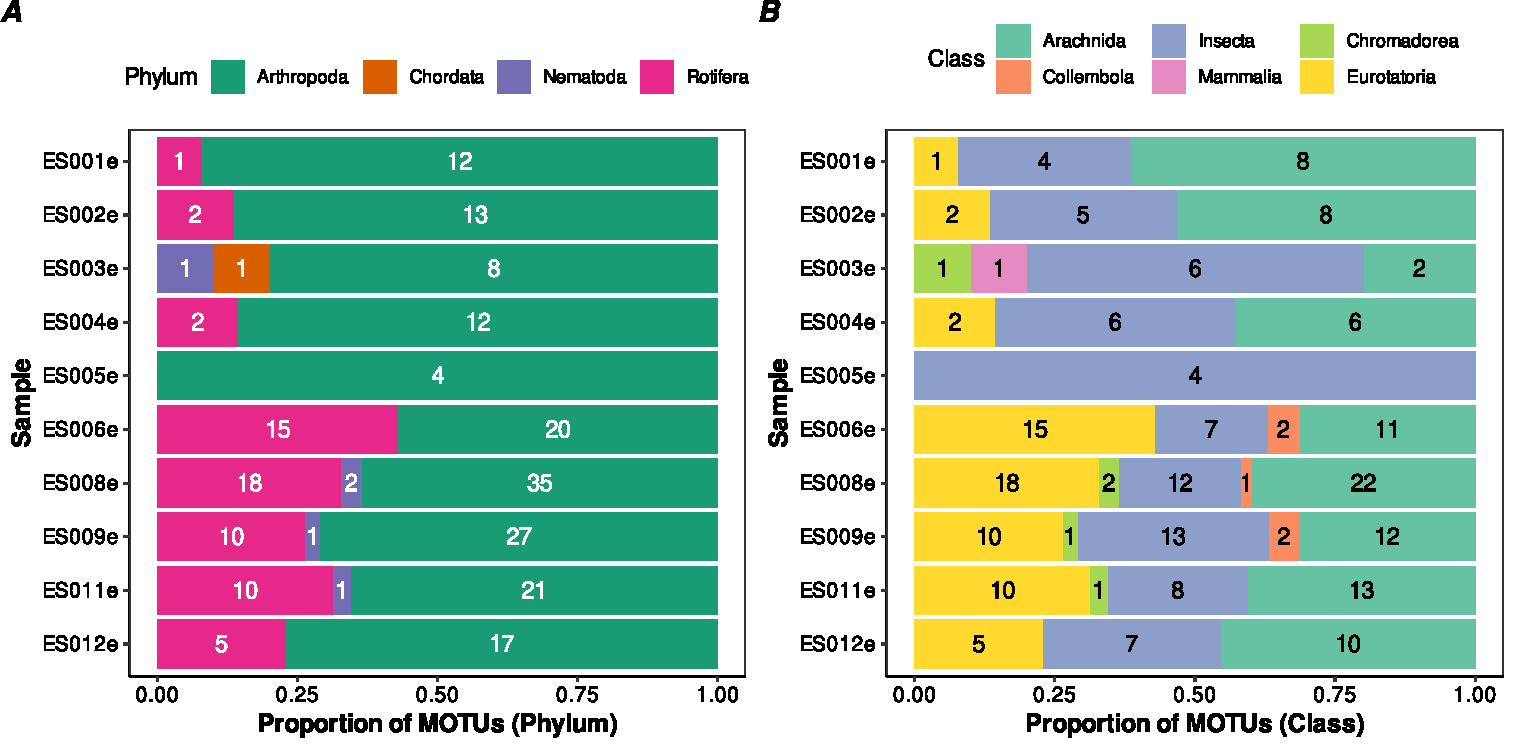
\includegraphics[width=\linewidth]{figures/05_motus.pdf}
    \caption{Proportion of molecular operational taxonomic units (MOTUs) within each sample classified by Phylum (A) and Class (B). Numbers refer to the absolute number of \glspl{MOTU}. \gls{eDNA} analyses with COI recovered mainly Arthropoda and in particular Insecta and Arachnida.}
    \label{fig:5-barplot}
\end{figure*}
% \end{figure}

A total of $\sim$13.6 million reads were obtained from the first flow cell containing both short and long COI libraries, and $\sim$3.19 million reads from the second flow cell containing only the 658 bp library. A total of $\sim$3.46 and $\sim$2.16 million reads were demultiplexed for the 658 and 313 bp libraries, respectively. The number of reads demultiplexed per sample per primer dataset can be found in Supplementary Figure~\ref{fig:s3-reads} and File~S1. Amplicon\_sorter generated a total of 9,403 consensus sequences across all samples and primer datasets, which was further collapsed to 4,048 \glspl{MOTU} at the 3\% p-distance threshold. 2,129 \glspl{MOTU} had a BLAST hit at $\geq 85 \%$ sequence similarity and $\geq 85 \%$ query cover. Finally, after filtering away non-Metazoa \glspl{MOTU} and \glspl{MOTU} found in the sample blank, we retained 152 metazoan \glspl{MOTU} from across 10 samples (Supplementary File S2). No \glspl{MOTU} were found in the PCR negatives, while the sample blank (ES000b) contained only non-Singapore taxa.

The 152 metazoan \glspl{MOTU} detected were mainly invertebrates classified to phylum Arthropoda, Rotifera, and Nematoda. We only detected a single chordate \gls{MOTU}, since the COI short primers were designed to target metazoan invertebrates \cite{leray-2013,lobo-2013}. Arthropoda was the most abundant phylum detected at the sample level, and across the entire dataset (Fig.~\ref{fig:5-barplot}A), followed by Rotifera, Nematoda, and Chordata. Notable taxa detected included arboreal organisms like the long-tailed macaque (\textit{Macaca fascicularis}), multiple ant and termite species (\textit{Camponotus} sp., \textit{Crematogaster} sp., \textit{Hospitalitermes} sp.), and even organisms that feed on plants (e.g., gall midges, \textit{Cecidomyiidae} sp.). Within Arthropoda, \glspl{MOTU} were evenly split between Arachnida and Insecta, although Collembola was occasionally detected in night samples (Fig.~\ref{fig:5-barplot}B). %
% Additional info on soil animals
Most probes indicate signals of soil-associated organisms. Notably, probes ES0006e, ES0008e, and ES0009e all contain Collembola, corroborating that these probes reached the forest floor, as Collembola are known soil-associated organisms. However, it is important to note that the tree canopy and forest floor environment are not mutually exclusive. Many animals, such as birds, reptiles, squirrels, and non-human primates, like the long-tailed macaque, inhabit both ground and arboreal environments. Consequently, it is expected to find soil organisms in swabs collected from tree top canopies and vice versa.
%
The detection of arboreal species from our samples demonstrates the potential of the eProbe for surface \gls{eDNA} collection from forest canopies. 
Future studies could incorporate a targeted metabarcoding approach, which involves the use of a suite of primers to target specific types of arboreal taxa that were not detected with the COI primers. Examples include MiMammal \cite{ushio-2017} or MiBird and BirdT \cite{ushio-2018, thalinger-2023} primers to improve detection of mammals and birds, respectively. As nanopore sequencing is not limited by length, other mitochondrial genes could be targeted, such as Cytochrome b, which have more reference data available for vertebrates, but have been limited in use for \gls{eDNA} metabarcoding due to the length needed for sequencing.

iNEXT rarefaction analysis suggests that approximately 75 probes are needed to reach an asymptote and fully capture the metazoan \gls{MOTU} richness of the sampled area (Supplementary Fig.~\ref{fig:s4-accumulation}). This scenario highlights the potential advantages of drone-based \gls{eDNA} sampling in reducing sampling effort and associated risks. Considering the average sampling time of 12.5 minutes for the eProbe, it is projected that approximately 21 hours of sampling duration would be necessary to achieve the asymptote. To reach this sampling duration, measures should be taken to minimize downtime associated with breaks required for the drone operator's rest. This could be facilitated through further automation via pre-programmed flight paths. Additionally, pre-mapping the forest using RGB images or LIDAR point clouds to pinpoint denser canopies could potentially enhance \gls{eDNA} concentration per sample and mitigate the pronounced variability observed in current samples (Table~\ref{tab:1-metadata}, Supplementary Fig.~\ref{fig:s5-dbra}), thus reducing the number of required samples. Lastly, by optimizing the molecular tools to be focused on specific targets, we could increase detection rate per sample and decrease sampling effort. As nanopore technology improves, using genetic markers with longer reads enables new \gls{eDNA} metabarcoding protocols. We know that \gls{eDNA} is not significantly degraded in water when the species are present as it has been demonstrated that whole mitochondrial genomes are possible to amplify using long-range PCR \cite{deiner-2017}. While we need to test whether DNA remains unfragmented in surface samples, many optimizations can be made beyond this proof of concept to improve both on the robotic collection and the molecular protocols employed.

% \begin{figure}[tb]
\begin{figure*}[tb]
    \centering
    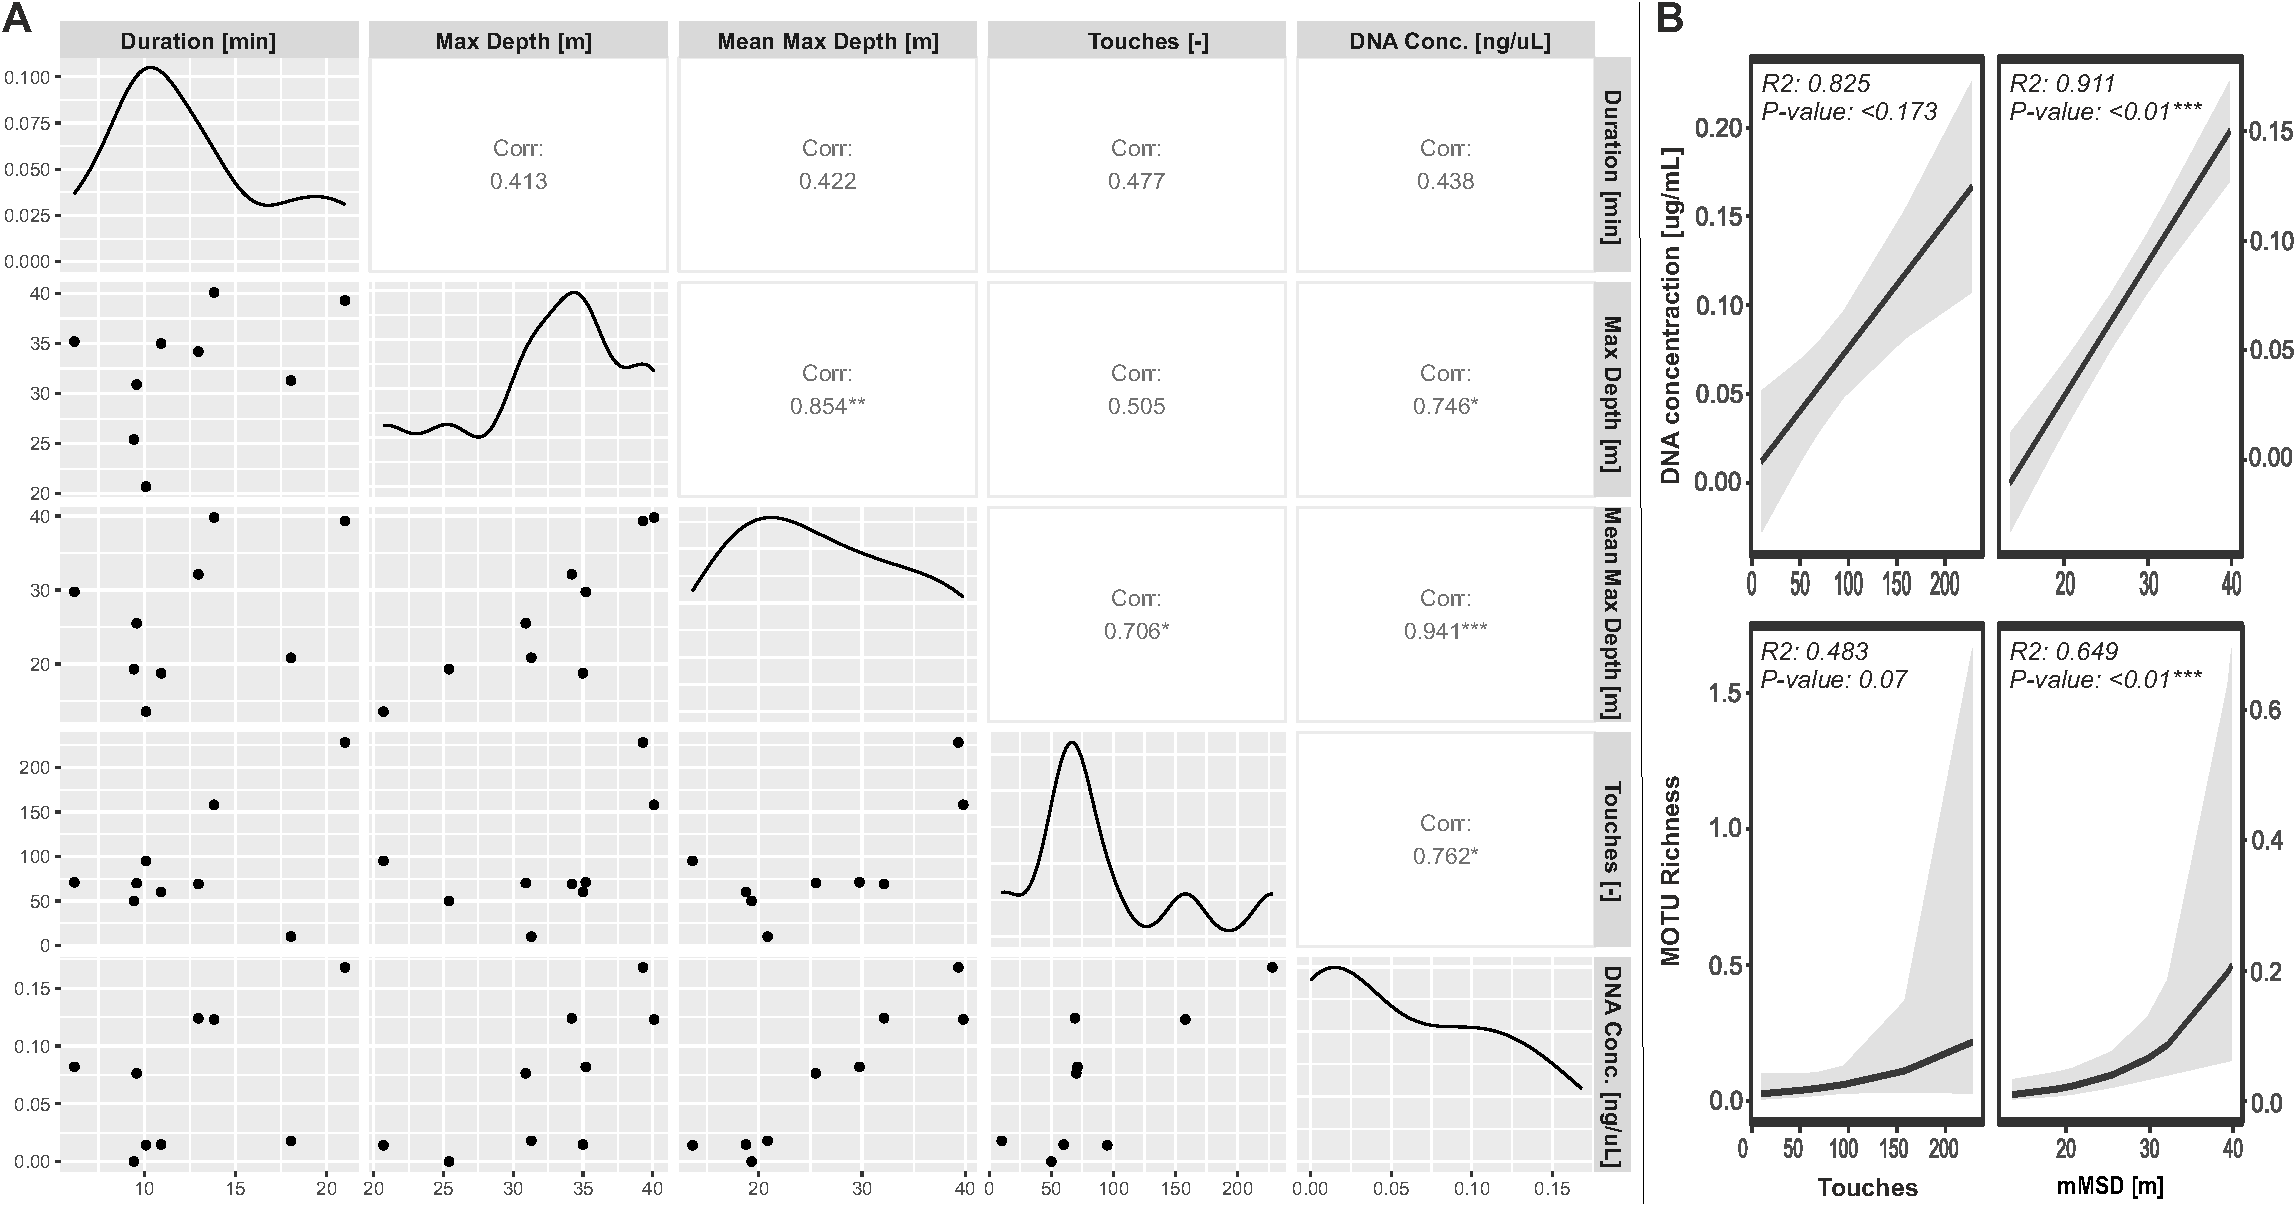
\includegraphics[width=\linewidth]{figures/06_corr.pdf}
    \caption{(A) Density plots (diagonal) and correlation of each variable (scatterplot and statistics respectively below and above the diagonal). (B) Results of the generalized linear model for the predicted DNA concentration and \gls{MOTU} richness for the number of touches and the mean maximum sampling depth (mMSD). In each plot, the R2 of the model and P-values relative to the variable tested are reported. *, ** and *** denote statistical significance levels of 0.05, 0.01 and 0.001.}
    \label{fig:6-corr}
\end{figure*}
% \end{figure}

To understand the factors impacting the drone-assisted sample collection, we performed a correlation analysis using the sample metadata (Table~\ref{tab:1-metadata}) and focused on \gls{eDNA} concentration as a proxy for the performance of sample collection (Fig.~\ref{fig:6-corr}). The main observed variables include sampling duration, maximum depth (from UAV altitude), the mean maximum depth and the number of touches. Apart from maximum depth and mean maximum depth, the variables do not show a high correlation. The DNA concentration was positively correlated with the number of touches and the mean maximum depth (Fig.~\ref{fig:6-corr}). This correlation was also partially confirmed by the \glspl{GLM} that retrieved a significant effect (R2: 0.911, p-value < 0.01) of the mean maximum depth (Fig.~\ref{fig:6-corr}). A deeper sampling depth may be associated with higher number of habitats sampled, crossing the canopy, the understory and even reaching the ground in some cases. This seems to be more important than the number of times any surface was touched, supporting the result of the rarefaction curve and the need of a higher number of samples in general.

The PERMANCOVA showed a significant effect (R2: 0.16, p-value < 0.01) of the DNA concentration over the community composition but not of the time (Supplementary Table~\ref{tab:s1-permancova}). From the dbRDA the mean maximum depth and the duration of the sampling were the two most important variables, together with the DNA concentration, responsible for the differences between the species detected in each sample.

%%%%%%%%%%%%%%%%%%%%%%%%%%%%%%%%%%%%%%%%%%%%%%%%%%%%%%%%%%%%%%%%%%%%%
%% Discussion
%%%%%%%%%%%%%%%%%%%%%%%%%%%%%%%%%%%%%%%%%%%%%%%%%%%%%%%%%%%%%%%%%%%%%
\section{Outlook and Implications}
\label{sec:outlook}

Our study proposes a drone-based sampling methodology to collect \gls{eDNA} from tree canopies through surface swabbing. During the XPRIZE Rainforest Semi-Finals, we demonstrated the efficacy of this approach by collecting ten samples in both day and night, and subsequently identifying 152 metazoan \glspl{MOTU} spanning six classes of taxonomic diversity with nanopore sequencing technology. The small amount of effort and time to survey such a diverse community of species is a major improvement for using eDNA in such settings. Our in-field verification therefore provides a proof of concept for the eProbe’s capacity to survey terrestrial biodiversity in rainforests. This serves as an important step forward, as much of the world's undiscovered and often threatened biodiversity can be found in these remote and inaccessible habitats.

%old
%Our study proposes a drone-based sampling methodology to collect \gls{eDNA} from tree canopies. By safely hovering above the forest canopy and employing a probe equipped with \gls{eDNA}-retaining material, this method optimizes surface swabbing techniques to collect genetic traces directly from tree branches and leaves from the forest canopy to the forest floor. During the XPRIZE Rainforest Semi-Finals, we demonstrated the efficacy of this approach by collecting ten samples in both day and night, and subsequently identifying 152 metazoan \glspl{MOTU} spanning six classes of taxonomic diversity with nanopore sequencing technology. The small amount of effort and time to survey such a diverse community of species is a major improvement for using \gls{eDNA} in such settings. The work here demonstrates some key correlations in the depth and the number of touches of the eProbe into the canopy. Our in-field verification therefore provides a proof of concept for the eProbe’s capacity to survey terrestrial biodiversity in rainforests. This serves as an important step forward, as much of the world's undiscovered and often threatened biodiversity can be found in these remote and inaccessible habitats.

To fully harness the benefits of drone-based surface \gls{eDNA} collection, further advancements in both robotics and \gls{eDNA} analysis protocols are essential. The integration of autonomous drone operations presents an important aspect to extend sampling range and reduce downtime. To achieve autonomous operation, the robotic system needs to be robustified and probe entanglement reduced through further optimization of system parameters. Furthermore, determining  an optimal sampling strategy, including when, where and for how long to collect surface \gls{eDNA} to capture a representative picture of biodiversity becomes imperative.
In the field of \gls{eDNA} metabarcoding, further research and development is needed to establish the full pipeline of in-field \gls{eDNA} analysis from extraction to sequencing and bioinformatics. Although portable sequencing technologies like the MinION were applied in this study, the heavy reliance on powered instruments for library preparation and the computational requirements needed for basecalling and bioinformatics continue to hamper a fully in-field sample-to-sequence eDNA-based workflow. Nanopore sequencing also opens up unexplored molecular protocols for \gls{eDNA} metabarcoding of sequencing longer reads for greater taxonomic and phylogenetic information. The future of \gls{eDNA} research should therefore focus on utilizing this capacity to design more fit-for-purpose and accessible protocols unlimited by sequence length and costly instruments for the detection and discovery of biodiversity. These activities will support the Nagoya Protocol \cite{nagoya} to enable fair and equitable sharing of benefits from genetic resource utilization and, more importantly, it will give agency to indigenous communities, who steward much of the world's biodiverse places. 

As so many ecosystems remain poorly studied, their loss may go largely unnoticed and we may even miss unprecedented change simply because we cannot measure it. The integration of robotic solutions with \gls{eDNA} sampling systems holds immense potential to provide baseline data on animal, plant, and microbial communities across large scales. The technology, from sampling to data processing, must progress concurrently to optimize biodiversity surveys comprehensively. This collaborative effort is timely and critical, considering the pressing need for scalable and cost-effective solutions for biodiversity monitoring in conservation and restoration initiatives.

%%%%%%%%%%%%%%%%%%%%%%%%%%%%%%%%%%%%%%%%%%%%%%%%%%%%%%%%%%%%%%%%%%%%%
%% The same is true for Supporting Information, which should use the
%% suppinfo environment.
%%%%%%%%%%%%%%%%%%%%%%%%%%%%%%%%%%%%%%%%%%%%%%%%%%%%%%%%%%%%%%%%%%%%%
\begin{suppinfo}

The supporting information is available free of charge:
\begin{itemize}
  \item Video\_Demonstration\_eProbe.mp4 (Video File, mp4) - Demonstration of the drone-based sample collection in the rainforest.
  \item Supplementary\_Figures\_and\_Tables.pdf (PDF File) - Additional information on sampling (control GUI, sampling locations, sample metadata) and DNA analysis (PERMANCOVA, demultiplexed reads, species accumulation curve, dbRDA)
  \item Supplementary\_File\_S1.XLSX (MS Excel Spreadsheet) - Nanopore run statistics, including tag combinations for demultiplexing PCR replicates.
  \item Supplementary\_File\_S2.XLSX (MS Excel Spreadsheet) - Taxonomic classifications of MOTUs found in this study, including the 152 metazoan MOTUs analyzed (“MOTUs\_Metazoa\_analysed”), and MOTUs omitted (“MOTUs\_non-Metazoa” and “MOTUs\_omitted”). 
\end{itemize}

The basecalled fastq files have been uploaded to NCBI’s Sequence Read Archive under BioProject PRJNA1090646. Raw pod5 files can be made available upon request. 
%Supplementary File S1 contains the nanopore run statistics, PCR demultiplexing information, reads demultiplexed, number of consensus sequences after amplicon\_sorter, and taxonomic classifications of metazoan \glspl{MOTU}.

\end{suppinfo}

%%%%%%%%%%%%%%%%%%%%%%%%%%%%%%%%%%%%%%%%%%%%%%%%%%%%%%%%%%%%%%%%%%%%%
%% Funding
%%%%%%%%%%%%%%%%%%%%%%%%%%%%%%%%%%%%%%%%%%%%%%%%%%%%%%%%%%%%%%%%%%%%%

\section*{Funding Sources}

This work was funded by the Swiss National Science Foundation under Eccellenza Grant (Grant Agreement No. 186865) and Bridge Discovery Grant (Grant Agreement No. 203550), and the European Research Council (ERC) under the European Union's Horizon 2020 research and innovation program (Grant Agreement No. 852621). It was further supported by the Rütli-Stiftung, the ETH Foundation, the XPRIZE Foundation and the Alana Foundation due to the participation of the authors in the XPRIZE Rainforest competition.

%%%%%%%%%%%%%%%%%%%%%%%%%%%%%%%%%%%%%%%%%%%%%%%%%%%%%%%%%%%%%%%%%%%%%
%% The "Acknowledgement" section can be given in all manuscript
%% classes.  This should be given within the "acknowledgement"
%% environment, which will make the correct section or running title.
%%%%%%%%%%%%%%%%%%%%%%%%%%%%%%%%%%%%%%%%%%%%%%%%%%%%%%%%%%%%%%%%%%%%%
\begin{acknowledgement}

The authors thank the Zoo Zürich, the XPRIZE Foundation and the National Parks Board, Singapore. We thank Eppendorf for the donation for in kind equipment and consumables and Patagonia for the backpack and sleeves for carrying our portable lab equipment to the field. We also thank Danwei Huang for permitting access to his laboratory for molecular work, and the National Supercomputing Centre (NSCC), Singapore, for permitting use of their computational resources for eDNA analysis. We also thank Gian Andri Morf and Andri Bisaz for initial work on the winch and probe system.  We also thank our entire XPRIZE Rainforest team ETH BiodivX for the collaborative spirit and feedback during the development of our solutions to improve biodiversity discovery and monitoring of rainforest.

\end{acknowledgement}

%%%%%%%%%%%%%%%%%%%%%%%%%%%%%%%%%%%%%%%%%%%%%%%%%%%%%%%%%%%%%%%%%%%%%
%% Notes (Conflict of interest
%%%%%%%%%%%%%%%%%%%%%%%%%%%%%%%%%%%%%%%%%%%%%%%%%%%%%%%%%%%%%%%%%%%%%
\section*{Conflict of Interest}

\normalsize
%
M.L. and L.P. cannot provide the exact methodology for the extraction method because it is planned to be part of a commercial offering. E.M and K.D. own a company that offers services for environmental DNA in a commercial setting. We further declare that the methodology and device of the eProbe surface swabbing has a patent pending under the application number 102023000011244.
%
%
%%%%%%%%%%%%%%%%%%%%%%%%%%%%%%%%%%%%%%%%%%%%%%%%%%%%%%%%%%%%%%%%%%%%%
%% The appropriate \bibliography command should be placed here.
%% Notice that the class file automatically sets \bibliographystyle
%% and also names the section correctly.
%%%%%%%%%%%%%%%%%%%%%%%%%%%%%%%%%%%%%%%%%%%%%%%%%%%%%%%%%%%%%%%%%%%%%
\footnotesize% make footnotesize
\bibliography{references}
%
%
%%%%%%%%%%%%%%%%%%%%%%%%%%%%%%%%%%%%%%%%%%%%%%%%%%%%%%%%%%%%%%%%%%%%%
%% The "tocentry" environment can be used to create an entry for the
%% graphical table of contents. It is given here as some journals
%% require that it is printed as part of the abstract page. It will
%% be automatically moved as appropriate.
%%%%%%%%%%%%%%%%%%%%%%%%%%%%%%%%%%%%%%%%%%%%%%%%%%%%%%%%%%%%%%%%%%%%%
%
\begin{tocentry}
%
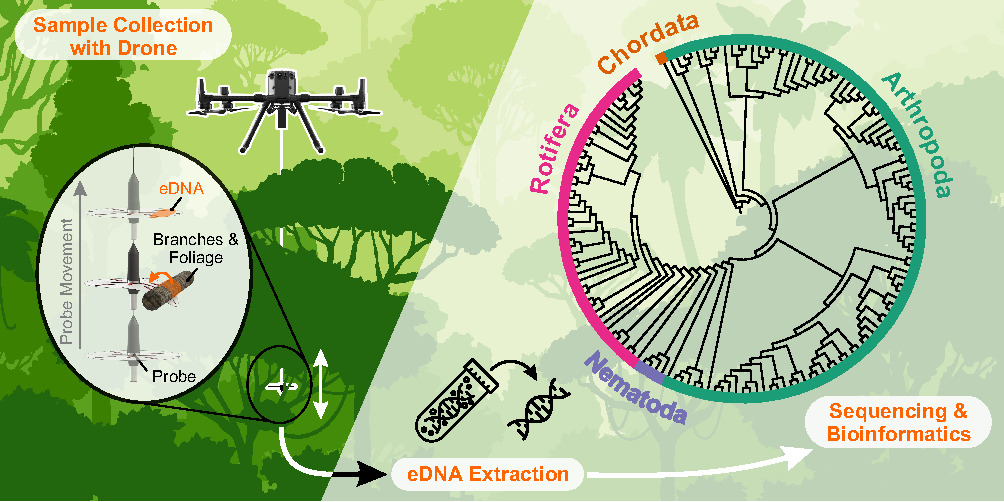
\includegraphics[width=\linewidth]{figures/00_graphical_abstract.pdf}
%
% Some journals require a graphical entry for the Table of Contents.
% This should be laid out ``print ready'' so that the sizing of the
% text is correct.
%
% Inside the \texttt{tocentry} environment, the font used is Helvetica
% 8\,pt, as required by \emph{Journal of the American Chemical
% Society}.
%
% The surrounding frame is 9\,cm by 3.5\,cm, which is the maximum
% permitted for  \emph{Journal of the American Chemical Society}
% graphical table of content entries. The box will not resize if the
% content is too big: instead it will overflow the edge of the box.
%
% This box and the associated title will always be printed on a
% separate page at the end of the document.
%
\end{tocentry}

\end{document}